\chapter{Enfoc}
\label{cha:enfoc}

En aquest capítol es descriu l'estratègia emprada per a resoldre l'algorisme tot formalitzant matemàticament els conceptes que hi intervenen. El primer apartat presenta l'estructura general de l'algorisme i els següents apartats aprofundeixen en cadascun dels mòduls que el formen.

\section{Estructura general de l'algorisme}

L'objectiu de l'algorisme es donar una mesura de similaritat entre un model BPMN i la descripció textual d'un procés. Per fer-ho, es segueix l'estructura de la figura \ref{fig:estructura}. L'objectiu és trobar quines frases del text i quines tasques del model estan relacionades per poder analitzar si aquesta relació presenta algun problema: Tasques del model que no es mencionen al text o viceversa, i casos en que l'ordre relatiu dels events no és el mateix.

A grans trets, l'informació del text i del model es parteix en unitats més simples. Posteriorment, se'n fa una extracció de característiques creant una representació uniforme pels elements del text i els del model. Tot seguit s'estableix una mesura de similaritat entre aquests elements. Paral·lelament, s'estableix un ordre parcial pels elements del text i els elements del model. Finalment tota aquesta informació --La similaritat i l'ordre entre elements-- es fa servir per calcular la correspondència òptima de tasques a frases. En els següents apartats s'explica formalment i amb més detall l'enfoc plantejat per a cadascuna d'aquestes parts.

\begin{figure}[!hbt]
    \includegraphics[width=\textwidth]{diagrams/Enfoc_Diagrama.png}
    \caption{Esquema de l'estructura de l'algorisme.}
    \label{fig:estructura}
\end{figure}

\section{Dades d'entrada}

Per tal de comparar el model BPMN amb el text, cal partir aquests en elements més simples. S'ha escollit dividir el text en frases i el model BPMN en tasques. 

Partir el text en tasques és l'alternativa més evident pel cas que ens plantegem, no obstant això trobem moltes vegades casos on la frase no és la unitat òptima. Considerem la frase: ``The chef prepares the meal and places it in the service hatch''. Aquesta frase conté la descripció de dues accions clarament diferenciades, \emph{``Prepare Meal''} i \emph{``Place it (meal)''}. Aquesta partició més fina es correspondria a partir la frase en \emph{predicats}, no obstant s'ha escollit simplificar el problema i considerar el text com una llista de frases.

D'altra banda, partir el model en tasques és una alternativa d'entrada contraintuitiva. En un model BPMN les tasques juguen un paper molt important, però hi ha altres elements que aporten bona part del significat: Les \emph{swimlanes} i \emph{pools}, les \emph{gateways} i el propi flux d'execució. De fet, l'enfoc no és considerar les tasques aïllades, sinó les tasques i el seu entorn. Així doncs, a l'hora de considerar la tasca \emph{``Clarify Shipment Method''} en la figura \ref{fig:exemple_secretary}, no només ens fixarem en el text de la tasca sinó que es considerarà també coses com que la \emph{swimlane} conté el text \emph{``secretary''}. Així evitem no perdre informació a l'hora de considerar el model.

\begin{figure}[!htb]
    \centering
    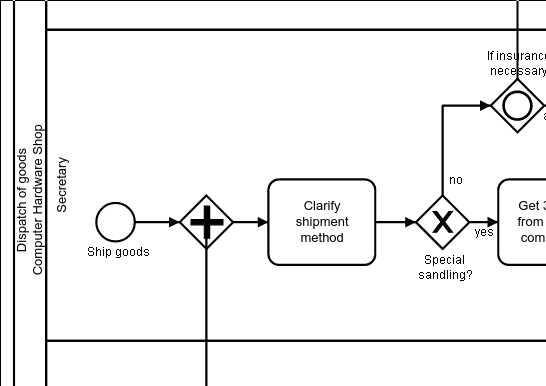
\includegraphics[width=0.7\textwidth]{figures/exemple-secretary.png} 
    \caption{Exemple il·lustratiu d'un fragment de model BPMN}
    \label{fig:exemple_secretary}
\end{figure}

Així doncs, definim l'entrada de l'algorisme com un conjunt $S = \{s_1, ..., s_N\}$ de frases i un conjunt $T = \{t1, ..., tM\}$ de tasques. Definim informalment els elements dels conjunts seguint la definició que hem donat en aquest apartat.

\section{Extracció de característiques}
\label{sec:enfoc-extraccio}

Com que les frases i les tasques son representacions d'informació totalment diferents, és difícil calcular directament la similaritat entre aquestes. Els càlculs estarien plenes de casos especials tenint en compte informació molt concreta dels dos costats. És per això que s'ha afegit un pas d'extracció de característiques, convertint els diferents elements en una representació comuna tant per tasques com per frases: els vectors de característiques.

Per a aquest projecte s'ha escollit un espai molt gran, potencialment infinit, de característiques $F = {f1, f2, ...}$ del tipus binari. Cadascuna d'aquestes característiques representa la presència d'algun atribut distintiu de l'objecte al que representa. Per exemple, la frase \emph{``The employee hands over his meal''} té la característica ``El subjecte és employee'', o $subjecte\_es(employee)$. Cal fixar-nos però, que en un espai com aquest existeixen \emph{tipus} de característiques. Definim també el conjunt: $\{f(x) | x \in \Omega^n\}$ com el tipus de característica de f. Així doncs el tipus de característica $subjecte\_es$ conté característiques concretes com $subjecte\_es(employee)$ i $subjecte\_es(secretary)$. Cal notar com el valor $x$ d'una característica de tipus $f$ és una tupla ordenada de $n$ elements de qualsevol tipus. Aquest valor $n$ l'anomenarem \emph{aritat} del tipus de característica i depèn del tipus concret.

L'objectiu és representar les tasques i les frases com a vectors de característiques. A nivell teòric, un vector de característiques $v = [v_1, v_2, ..., v_n], v_i \in {0,1}$ té una dimensió per característica, amb un valor binari indicant si la característica és present en aquell objecte concret. Com que aquesta representació no és viable per al nostre espai de característiques, s'ha optat per representar el vector de característiques com un subconjunt de $F$ de les característiques concretes que tindrien valor 1 al vector de característiques. Aquesta representació és típica a la literatura quan l'espai de característiques és infinit. 

Definim finalment una funció extractora d'un tipus d'objecte $X$ com una funció $f_X: X \rightarrow \mathcal{P}(F)$\footnote{Amb $\mathcal{P}(F)$ em refereixo al \emph{powerset} de $F$, és a dir, tots els possibles subconjunts de característiques.}. En el domini d'aquest problema, definim les funcions extractores de manera diferenciada per les tasques i les frases. Així foncs tenim funcions extractores $f_{Task}$ i $f_{Sentence}$. Notar que les característiques que s'extreuen de les tasques i les frases són les mateixes, això és important a l'hora de comprar-les.

Formalment, l'extracció de característiques consisteix a convertir els conjunts $S$ i $T$ en els conjunts $S_{features}$ i $T_{features}$ de vectors de característiques. Definim $S_{features}$ com $\{f_{Sentence}(s) | s \in S\}$, i anàlogament pel cas de $T_{features}$.

\section{Càlcul de similaritat}
\label{sec:enfoc-similaritat}

Un cop hem reduït el problema de comparar frases i tasques a comparar vectors de característiques homogenis, calcular la similaritat entre aquests és un problema ben conegut a la literatura\cite{similarity}. Diferents tipus de dominis es beneficien més de diferents tipus de mètriques de similaritat. En aquest apartat considerem algunes de les mètriques més utilitzades en aquest àmbit que resultarien útils per a resoldre el problema.

\begin{description} 
    \item[Similaritat de cosinus]{Considerant els vectors de característiques com a vectors pròpiament dits, una dimensió per característica, aquesta mètrica considera dos vectors més similars com més petit és l'angle entre ells dos. Es fa servir el fet que $u \cdot v = |u| |v| cos(angle(u,v))$:$$Cosine(A, B) = \frac{A}{|A|} \cdot \frac{B}{|B|}$$ Aquesta mètrica dóna un valor acotat entre 0 i 1}
    \item[Índex de Jaccard]{Considerant els vectors de característiques com a conjunts d'aquestes, aquesta mètrica es calcula amb la fórmula: $$Jaccard(A,B) = \frac{|A\cap B|}{|A\cup B|}$$ Aquesta mètrica dóna un valor acotat entre 0 i 1.}
    \item[Índex de Jaccard ponderat]{Aquesta mètrica és una extensió de l'índex de Jaccard que considera una funció que assigna un pes a cada característica. El resultat dóna major importància a les característiques amb major pes: $$WeightedJaccard(A,B) = \frac{\sum_{x \in A\cap B}{weight(x)}}{\sum_{y\in A\cup B}{weight(y)}}$$ Aquesta mètrica també dona un valor acotat entre 0 i 1.}
    \item[Índex de Solapament\footnote{Traducció d'\emph{Overlapping Index}}]{Considerant els vectors de característiques novament com a conjunts, l'índex de solapament es calcula com $$Overlapping(A,B) = \frac{|A\cap B|}{min(|A|, |B|)}$$}
    \item[Índex de Solapament ponderat]{Similarment al cas de l'índex de \emph{Jaccard}, definim l'índex de solapament ponderat de la següent manera:$$WeightedOverlapping(A,B) = \frac{\sum_{x \in A\cap B}{weight(x)}}{\sum_{y\in shortest(A,B)}{weight(y)}}$$}
\end{description}

\section{Càlcul d'ordre}
\label{sec:enfoc-ordre}
En els apartats anteriors hem treballat partint el text i el model en objectes més petits: frases i tasques. Però a part de considerar aquests de manera separada, és molt important considerar l'estructura que els uneix. En el cas dels models BPMN la sequència de les tasques és clara i ve totalment determinada per l'estructura de graf del model. En canvi, pel text, detectar-ne l'estructura, o ordre en que succeeixen els events, és tot un problema en sí mateix. Aquest pas de l'algorisme correspon a, donats el text i el model BPMN inicials, derivar-ne un ordre parcial dels seus elements.

Més formalment, donats dós elements d'un dels dos conjunts $S$ i $T$, l'objectiu és trobar la relació $\rightsquigarrow$ que, per cada element de $S \times S$ o $T \times T$ indiqui si el primer element precedeix al segon.

\subsection{Al text}
\label{sec:enfoc-ordre-text}

Per poder calcular l'ordre entre els elements de $S$, és necessari fer una interpretació del temps a nivell temporal, detectant quines frases van abans d'altres a nivell cronològic. Tot i que aquest enfoc és possible\footnote{Cal dir que l'ambiguitat inherent al llenguatge natural fa que els resultats obtinguts amb aquest enfoc no siguin del tot exactes.}, queda fora de l'àmbit d'aquest projecte. Per aquest fet, hem considerat que l'ordre entre les frases del text és l'ordre d'aparició en aquest. És a dir, definim la relació d'ordre entre $s_i$ i $s_j$: $$s_i \rightsquigarrow s_j \iff i < j$$

Encara que d'entrada aquesta simplificació pugui semblar molt exagerada, cal considerar que estem tractant amb textos molt concrets. Les descripcions de procés són textos tècnics i en la seva redacció sempre és preferible la claredat. És per això que generalment es compleix aquesta propietat d'ordre.

\subsection{Al model}
\label{sec:enfoc-ordre-model}

En el model BPMN, per poder modelar millor aquesta relació d'ordre, adaptem la notació de graf de procés definida a \ref{behavioral_profiles}. Un graf de procés és una tupla $PM = (A, G, F, s, e, t)$ on:

\begin{itemize}
    \item[--] $A$ és el conjunt finit d'activitats, equivalent a $T$
    \item[--] $G$ és el conjunt finit de \emph{gateways}
    \item[--] $N = A\cup G$
    \item[--] $F$ és el conjunt d'arestes entre els elements del model BPMN.
    \item[--] $\bullet n = \{n' \in N | (n',n) \in F\}$ i $n\bullet = \{n' \in N | (n, n') \in \}$, conjunts de predecessors i successors.
    \item[--] $s \in A$, l'única activitat inicial. $\bullet s = \emptyset$.
    \item[--] $e \in A$, l'única activitat final. $e\bullet = \emptyset$.
    \item[--] $t : G \rightarrow \{and, xor\}$, funció que associa cada gateway a un tipus concret\footnote{Existeixen altres tipus de gateway en el formalisme del BPMN, aquests s'han de classificar en les categories $and$ o $xor$ en funció de si permeten l'execució simultània de múltiples branques o no.}.
\end{itemize}

Aquest formalisme és una simplificació de la notació BPMN, però és suficient per definir una estratègia algorítmica per determinar l'ordre entre els elements. A més, cal notar que un graf de procés i un model BPMN no són equivalents. En aquesta notació, un graf de procés és equivalent a una pool en un model BPMN (veure apartat \ref{introduccio-bpmn}).

Per completar la definició de l'ordre parcial, abans hem de definir les traces. Una traça en el model és una llista d'elements de $N$ de la forma $s \cdot A* \cdot e$ de manera que per cada parella de nodes consecutius $(n, n')$ en la llista tinguem que $(n, n') \in F$. Dit d'altra manera, una traça és un camí en el graf del model que va del node inicial al node final: Una possible execució del model. Definim el conjunt $\tau _{PM}$ com el conjunt de totes les possibles traces del model $PM$.

Així doncs, definim la relació $\preceq$ per a un procés $PM$ com el conjunt de parells $(x,y)$ de $(N\times N)$ tals que existeix una traça $\sigma = n_1, \cdots, n_m \in \tau _{PM}$ on $x=n_i$ i $y=n_j$ per dos naturals $i < j$ entre $1$ i $m$. O, en altres paraules, existeix una traça on x apareix abans que i.

I finalment, partint de la definició d'ordre parcial, podem establir les tres relacions que conformen el \emph{Behavioral Profile} d'un graf $PM$. Per cada parella de nodes $(x,y) \in N\times N$, $x$ i $y$ tenen una única d'aquestes relacions:
\begin{itemize}
    \item Ordre estricte: $x \rightsquigarrow _{PM} y \iff x \preceq y$ i $y \npreceq x$ 
    \item Ordre estricte invers: $x \leftsquigarrow _{PM} y \iff y \preceq x$ i $x \npreceq y$ 
    \item Exclusivitat: $x +_{PM} y \iff x \npreceq y$ i $y \npreceq x$.
    \item Paral·elisme: $x ||_{PM} y \iff x \preceq y$ i $y \preceq x$.
\end{itemize}

El behavioral profile d'un graf de procés és una informació molt important a l'hora de realitzar-ne un anàlisi, permetent trobar dependències entre tasques i determinar quines accions es poden dur a terme en paral·lel.

Veiem doncs com la relació que buscavem és un subconjunt del \emph{Behavioral Profile} del graf de procés del BPMN en questió. 

Tot i això, aquest enfoc només serveix per establir l'ordre entre els elements d'un graf de procés. Aquest projecte pretén analitzar qualsevol model bpmn, i els models amb múltiples pools defineixen múltiples grafs de procés per a un sol model, que es comuniquen a partir de message flows (veure apartat \ref{sec-introduccio-bpmn}. Com que aquest enfoc només té en compte els sequence flows --arcs en el graf de procés-- cal un postprocessat addicional per tenir en compte l'informació que ens proporcionen els missatges. 

Suposem que tenim un model BPMN amb diferents pools, o grafs de procés, $BPMN = {PM_1, \cdots, PM_K}$ i una conjunt de message flows $MF = \{(n_1, n_2) | n1 \in PM_i \land n_2 \in PM_j \land i \neq j\}$\footnote{En aquesta expressió s'utilitza $n \in PM$ per dir que $n$ pertany al conjunt de nodes de $PM$.}. A més, definim per a tot node $n$ els conjunts $After_n = \{n' \in N | n \rightsquigarrow n'\}$ i $After_n = \{n' \in N | n' \rightsquigarrow n\}$. El postprocessat correspon al següent algorisme:

\begin{enumerate}
    \item Creem un nou behavioral profile $BF$ amb els nodes de $PM_1 \cdots PM_K$, i considerem totes les relacions entre elements de diferents grafs de procés com a $+$.
    \item Per cada message flow $(n_i, n_j) \in MF$:
        \begin{enumerate}
            \item Modifiquem a $BF$ la relació entre $n_i$ i $n_a$ per $\rightsquigarrow$ per tot $n_a \in After_{n_j} \cup {nj}$
            \item Modifiquem a $BF$ la relació entre $n_j$ i $n_b$ per $\leftsquigarrow$ per tot $n_b \in Before_{n_i} \cup {ni}$
            \item Afegim tambés les relacions simètriques, si escau.
        \end{enumerate}
    \item Repetir el punt anterior fins que el behavioral profile convergeixi (no es modifiquen relacions noves)
\end{enumerate}

Aquest algorisme iteratiu permet crear un \textit{behavioral profile} general per a tot el model BPMN. Després del postprocessat, tenim un ordre definit entre tots els elements del BPMN. Cal notar, però, que no sempre es pot establir un ordre entre dos elements, els elements pels quals no s'ha pogut establir l'ordre tindràn la relació d'exclusivitat en acabar l'algorisme.

\section{Càlcul de la correspondència òptima}
\label{sec:enfoc-matching}

El pas final és obtenir la correspondència òptima entre frases del text i tasques del model BPMN. Similarment a \cite{el_paper}, definim la correspondència òptima com la funció $f_{CO} : T \rightarrow S$ que compleix:

\begin{itemize}
    \item Assignació total: El domini de $f_{CO}$ és $T$, és a dir, totes les tasques tenen imatge.
    \item Optimalitat: Es maximitza la suma $\sum_{t \in T}{S(f_{Task}(t), f_{Sentence}(f_{CO}(t)))}$, on $S$ és una de les funcions de similaritat de l'apartat \ref{sec:enfoc-similaritat}.
    \item Consistència d'ordre: $s = f_{CO}(t) \land s' = f_{CO}(t') \land t \preceq t' \implies s \preceq s'$.
\end{itemize}

D'entrada el fet d'assignar frases a tasques, i no a l'inrevés, pot semblar arbitrari. No obstant això, la idea que hi ha darrere té a veure amb l'estructura implícita dels models BPMN i els textos. Les tasques d'un model BPMN estan pensades per definir una única acció atòmica. D'altra banda, una frase en un text pot contenir la descripció de diverses accions, ja sigui mitjançant oracions coordinades o subordinades, o fins i tot amb informació implícita. És per aquest fet que s'ha escollit fer l'assignació de frases a tasques, ja que el cas més habitual serà que una frase pugui referir-se a més d'una tasca, mentre que el cas contrari és menys probable. Una tercera opció seria considerar, ja no una funció, sinó una llista de parelles frase-tasca. Així es contemplaria el cas d'una tasca referint-se a dues frases i viceversa. Aquest tercer enfoc, però, té l'inconvenient que la restricció d'optimització preferirà el màxim nombre de paraelles possibles, assignant totes les tasques a totes les frases.

És també important considerar si aquest conjunt de restriccions pot donar lloc a un problema irresoluble. Vegem que no es pot donar mai aquest cas:

\begin{proof}
Sigui $S = \{s_1, \cdots, s_N\}$, $T = \{t_1, \cdots, t_M\}$ una instància qualsevol del problema. Considerem l'assignació $f_C$ tal que $f_C(t) = s_N$, $\forall t \in T$. Aquesta assignació $f_C$ compleix les restriccións d'assignació total i consistència d'ordre, ja que d'una banda totes les tasques tenen imatge i  per altra banda $\forall t, t': f_C(t) \preceq f_C(t')$, ja que totes les tasques s'assignen a la mateixa frase. Si $f_C$ no compleix la restricció d'optimalitat, vol dir que existeix una $f_C' = f_{CO} \neq f_C$, altrament $f_C = f_{CO}$. Veiem, doncs, com sempre existeix una solució al problema. 
\end{proof}

